\subsection{Diseño del barrido}

Se perfilaron los siete kernels de dataset GPU (excluyendo
\texttt{gpu\_dgemm\_n4096}, calibrado contra una referencia de cuBLAS por
razones ya documentadas en el catálogo) con \texttt{ncu} bajo tres valores
de \texttt{--launch-count} (5, 20, 50), midiendo el FLOP/byte estimado en
cada caso. Al procesar los resultados se encontró y corrigió un error real
en el script de este barrido (no del instrumento de producción): la
reconstrucción del nombre de la métrica de FMA/suma/multiplicación para
precisión simple omitía el prefijo \texttt{f} (\texttt{..\_fma\_pred\_on}
en vez de \texttt{..\_ffma\_pred\_on}), lo que hacía que los seis kernels
FP32 del barrido reportaran FLOP/byte=0. Los datos crudos de \texttt{ncu} ya
estaban en disco, así que se corrigió re-parseando sin re-perfilar. Un
segundo problema, de datos y no de análisis, afectó a
\texttt{rodinia\_heartwall}: ver la Sección de hallazgos colaterales
(video sintético truncado) -- se resolvió re-generando el video y
re-perfilando ese kernel específicamente.

\subsection{Resultados}

La Figura~\ref{fig:ncu-convergence} y la Tabla~\ref{tab:ncu-convergence}
muestran el FLOP/byte estimado en función del número de lanzamientos
perfilados, junto con el número real de lanzamientos alcanzado (columna
$n$, limitado por cuántas veces el kernel realmente invoca su función
principal -- pedir más lanzamientos de los que el programa ejecuta no
produce más datos).

\begin{table}[H]
\centering
\caption{Convergencia de FLOP/byte vs. número de lanzamientos solicitados a \texttt{ncu}.}
\label{tab:ncu-convergence}
\small
\begin{tabular}{@{}lrrrr@{}}
\toprule
\textbf{Kernel} & \textbf{$n$ real (máx. 3 puntos)} & \textbf{OI a 5} & \textbf{OI a 20/10} & \textbf{OI a 50} \\
\midrule
\texttt{rodinia\_backprop} & 2 (fijo) & 0{,}07987 & 0{,}07987 & 0{,}07986 \\
\texttt{rodinia\_lavamd} & 1 (fijo) & 708{,}49 & 708{,}30 & 708{,}35 \\
\texttt{rodinia\_dwt2d} & 5 / 10 / 10 & 2{,}1762 & 2{,}1762 & 2{,}1741 \\
\texttt{rodinia\_hotspot} & 5 / 20 / 50 & 5{,}0232 & 5{,}0206 & 5{,}0200 \\
\texttt{rodinia\_heartwall} & 5 / 20 / 50 & 35{,}300 & 35{,}297 & 35{,}350 \\
\texttt{rodinia\_myocyte} & 5 / 20 / 50 & 0{,}01704 & 0{,}01692 & 0{,}01704 \\
\texttt{rodinia\_lud} & 5 / 20 / 50 & \textbf{7{,}492} & \textbf{7{,}584} & \textbf{7{,}668} \\
\bottomrule
\end{tabular}
\end{table}

\begin{figure}[H]
\centering
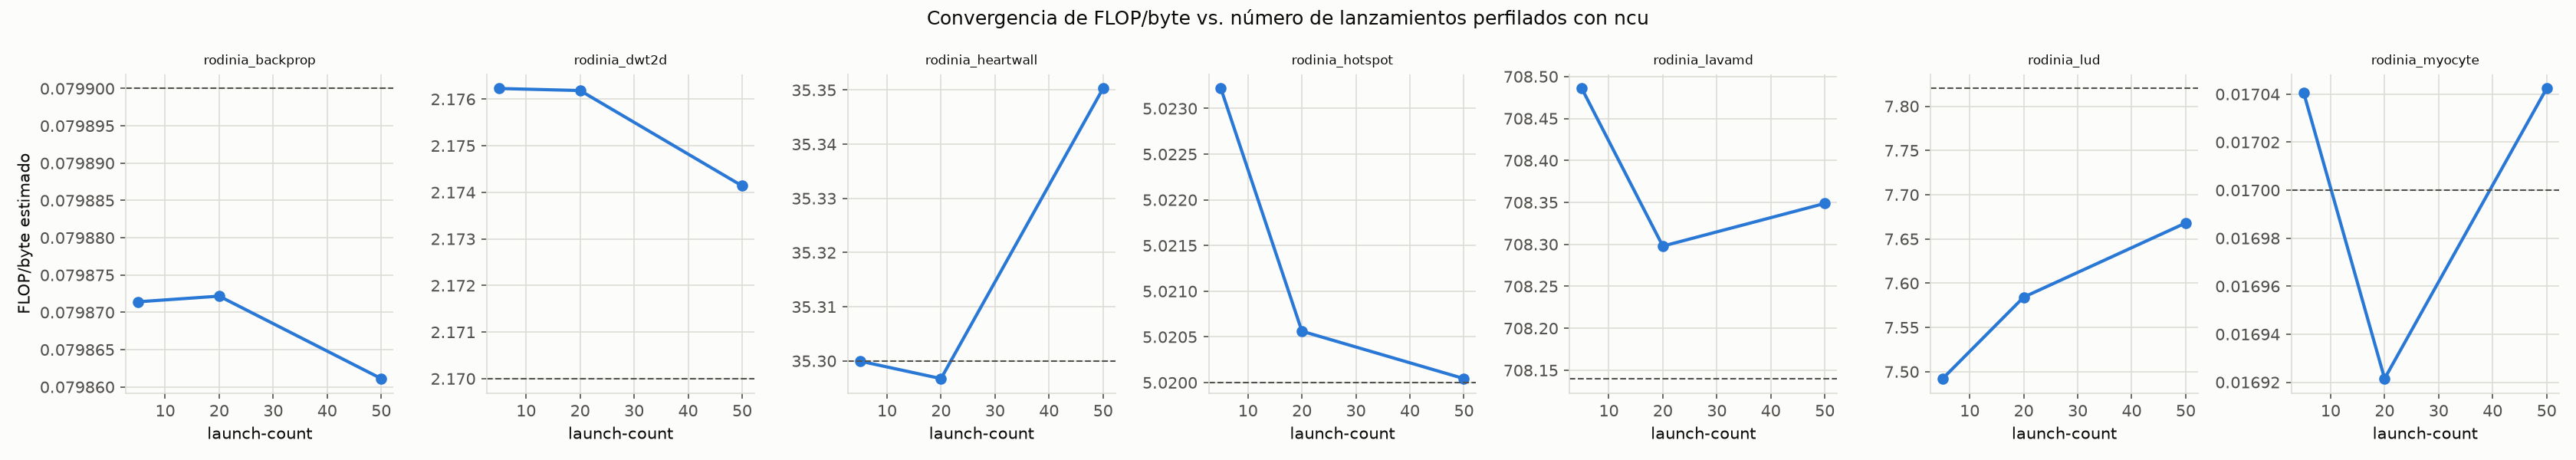
\includegraphics[width=\textwidth]{../plots/ncu_launch_count/ncu_convergence.png}
\caption{FLOP/byte estimado vs. lanzamientos solicitados, siete kernels de
dataset GPU. La línea punteada marca el valor declarado en el catálogo.}
\label{fig:ncu-convergence}
\end{figure}

Seis de los siete kernels no dejan nada que barrer de forma significativa:
\texttt{rodinia\_backprop} y \texttt{rodinia\_lavamd} solo tienen 2 y 1
lanzamiento real respectivamente (sin importar cuántos se soliciten, ya
está el dato completo desde el primer punto); \texttt{rodinia\_dwt2d} se
satura en 10 lanzamientos reales; y \texttt{rodinia\_hotspot},
\texttt{rodinia\_heartwall} y \texttt{rodinia\_myocyte} sí tienen
lanzamientos de sobra pero su FLOP/byte ya es estable dentro de
$\pm$ 0{,}2\,\% desde 5 lanzamientos.

\textbf{\texttt{rodinia\_lud} es la única excepción real}: con lanzamientos
de sobra disponibles, el FLOP/byte estimado sube de forma monótona y no
plateada entre 5 y 50 lanzamientos (7{,}49 $\to$ 7{,}58 $\to$ 7{,}67, una
variación de +2{,}3\,\% sin señal clara de haber convergido en el
extremo superior del rango probado). Esto es significativo precisamente
porque \texttt{rodinia\_lud} es el único kernel del catálogo etiquetado
``intermedio'': su intensidad operacional declarada (7{,}82 FLOP/byte,
ARC-80) queda apenas un 7{,}4\,\% por encima del \emph{ridge} FP32
vainilla medido en este mismo nodo con el probe propio del proyecto
($\approx$7{,}28 FLOP/byte, ARC-76 -- corrección respecto a un valor de
7{,}98 usado en una versión anterior de este análisis, que no correspondía
a ninguna medición del catálogo). Con ese ridge correcto, los tres puntos
de este barrido (7{,}49 a 7{,}67) ya están por \emph{encima} del ridge
desde el primer punto (5 lanzamientos) -- la clasificación
\texttt{compute\_bound} no cambia en el rango medido, pero el margen sobre
el ridge sí cambia de forma sustancial según cuántos lanzamientos se usen
(de 2{,}9\,\% de margen a 5 lanzamientos hasta 4{,}9\,\% a 50), lo cual
importa precisamente porque el caso es borderline por diseño (menos del
8\,\% de margen incluso en el valor ya declarado). Con solo estos tres
puntos, lo único que puede afirmarse es que 50 lanzamientos son
insuficientes para estabilizar ese margen -- no que 200 (el valor ya
declarado en el catálogo, ARC-80) sean el número correcto; extrapolar esa
suficiencia sin medirla sería precisamente el tipo de afirmación
sobredimensionada que este informe busca evitar.

\subsection{Extensión dirigida: cerrando la convergencia de \texttt{rodinia\_lud}}

Se perfilaron tres puntos adicionales para este kernel específicamente
(100, 150 y 200 lanzamientos, 3 corridas de \texttt{ncu} de costo bajo),
aplicando un criterio de convergencia declarado \textbf{antes} de ver el
resultado: convergencia = cambio relativo menor al 1\,\% entre cada par
consecutivo de puntos.

\begin{table}[H]
\centering
\caption{Convergencia extendida de \texttt{rodinia\_lud} (criterio: $\Delta < 1$\,\% pre-declarado).}
\label{tab:lud-convergence-extended}
\small
\begin{tabular}{@{}lrr@{}}
\toprule
\textbf{Lanzamientos} & \textbf{FLOP/byte} & \textbf{Cambio relativo vs. punto anterior} \\
\midrule
5   & 7{,}4922 & -- \\
20  & 7{,}5842 & 1{,}23\,\% \\
50  & 7{,}6680 & 1{,}11\,\% \\
100 & 7{,}7737 & 1{,}38\,\% \\
150 & 7{,}8162 & \textbf{0{,}55\,\%} (converge) \\
200 & 7{,}8240 & 0{,}10\,\% \\
\bottomrule
\end{tabular}
\end{table}

\begin{figure}[H]
\centering
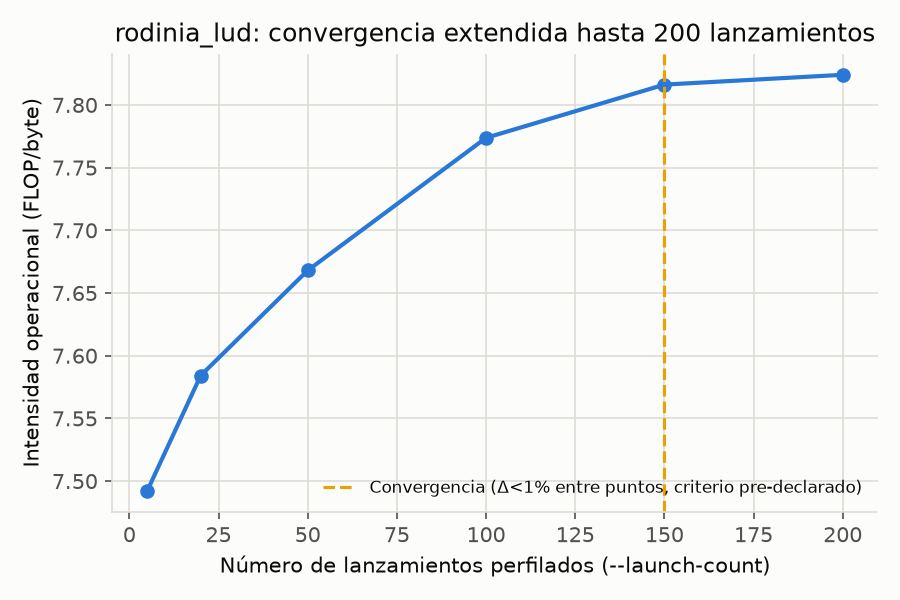
\includegraphics[width=0.75\textwidth]{../plots/lud_ncu_convergence_extended.png}
\caption{Convergencia extendida de \texttt{rodinia\_lud} hasta 200 lanzamientos.}
\label{fig:lud-convergence-extended}
\end{figure}

Con el criterio pre-declarado, la convergencia se alcanza en
\textbf{launch-count=150} (cambio de 0{,}55\,\% respecto al punto
anterior, y de solo 0{,}10\,\% entre 150 y 200). El valor de 200 usado en
el catálogo (ARC-80) queda ahora \textbf{confirmado con medición directa,
no solo con evidencia indirecta de no-convergencia a 50}: 200 lanzamientos
están efectivamente por encima del punto de convergencia real (150), con
un margen razonable, no arbitrariamente por encima de él.

\textbf{Conclusión}: no existe un número de lanzamientos único
correcto para todo el catálogo -- el número real de lanzamientos que cada
kernel ejecuta varía en más de dos órdenes de magnitud (de 1 a cientos), y
la velocidad de convergencia del FLOP/byte estimado varía igual de fuerte.
La práctica correcta, confirmada por este barrido, es perfilar con
suficientes lanzamientos para observar la meseta de convergencia
\emph{de cada kernel individualmente}, aplicando un criterio de
convergencia declarado de antemano -- para los seis kernels estables desde
5 lanzamientos, la evidencia ya alcanza para cerrar el parámetro; para
\texttt{rodinia\_lud}, el caso más exigente, la extensión a 200
lanzamientos cierra el parámetro con el mismo estándar de evidencia, en
vez de con una extrapolación razonable pero no medida.
